\section{Estimator} \label{sec:estimator}
The state estimation algorithm is responsible for accurately determining the current rocket state.
The rocket state is a set of data points which describe the condition of the rocket dynamics, and is made up of the rocket attitude, velocity, altitude, aerodynamic coefficients (coefficients are not quite certain due to the lack of available windtunnel testing) and other air data.
As the underlying dynamics are nonlinear in some cases, an \textit{Extended Kalman Filter} (EKF) is used to estimate the current state. The EKF algorithm uses these modelled dynamics to
\begin{enumerate}
    \item predict the current state from the last state and control inputs (desired canard angles) to the rocket, and then
    \item correct the state using measurements from onboard sensors, including rate gyroscopes, magnetometers, accelerometers, barometers.
\end{enumerate}
This whole process is a \textit{Bayes filter}, where the state estimate has an associated belief in the accuracy of the estimate.
Each iteration of the filter uses the the priori (old) state estimate and belief, to compute/update the posteriori (new) estimate and belief.


\subsection{Optimal estimation theory}
\label{sec:estimator_theory}
\textit{This section is here for completeness, it is not relevant for implementation.}
The system has continuous-time dynamics and discrete-time measurements \cite{lewis2008}
\begin{align}
    \dot x &= f(x, u, t) + w(t) \\
    y_k &= h(x_k,k) + v_k
\end{align}
where $w(t)$ is the process noise and $v_k$ is the measurement noise, which are additive, uncorrelated, and white zero-mean Gaussian processes \cite{lewis2008, werner2021b}. 
Both processes satisfy \cite{werner2021b} \footnote{Prof. Werner please forgive the butchering of the theory that is to follow}
\begin{align}
    \label{eq:estimator_theory_noise}
    E\left[ w(t) w^T(t+\tau) \right] &= Q_e \delta(t)
    &
    E\left[ v_{k} v^T_{k+1} \right] &= R_e \delta(k)
\end{align}
The estimation error $\varepsilon = x - \hat x$ is to be minimized in the cost function with weight vector $\varrho$ \cite{werner2021b}
\begin{equation}
    \min V = \lim_{t \to \infty} E\left[ \varepsilon^T \varrho \varrho^T \varepsilon \right]
\end{equation}
for which the solution is of the form \cite{werner2021b}
\begin{equation}
    V^* = \varrho^T P \varrho
\end{equation}
In infinite time, $P$ satisfies the filter algebraic Ricatti equation \cite{werner2021b}
\begin{equation}
    PF + F^TP - PH^TR_e^{-1}HP + Q_e = 0
\end{equation}
This results in the estimator feedback \cite{lewis2008}
\begin{align}
    \tilde x &= K_k \left[ y - h(\hat x_k) \right]
\end{align}
where the gain $K_k$ is computed with the a-priori covariance estimate $P_k^-$
\begin{align}
    K_{k} &= P_{k}^{-} H_k^T \left[ H_k P_{k}^{-} H_k^T + R_e \right]^{-1} 
\end{align}
(since the posteriori covariance $P_k$ is dependent on the current gain, the implicit equation would be $K_k = P_k^+ H_k^T R_e^{-1}$).

Due to the nonlinear behaviour of the state space functions, both $P$ and $K_k$ must be computed in real time as new measurements become available \cite{lewis2008}.
It is to note that the Kalman filter generally is only optimal for the mathematical model, not the actual plant (in this case the rocket) itself \cite{lewis2008}.
Additionally, the EKF is just quasi-optimal, as optimality is generally only proven for the case of linear state prediction and measurement functions.

\subsection{EKF algorithm}
The EKF thus propagates a state estimate $\hat x$ in discrete time steps, along with the belief in form of the covariance matrix $P$.
While the state is the mean estimate, the covariance matrix represents the ``uncertainty'' of the state estimate and their correlation, i.e. higher values represent more uncertainty. 

For its algorithm the EKF uses the continuous-time prediction model $f$ and the discrete-time measurement model $h$.
However, the EKF is running on a microprocessor in discrete time, so the continuous-time dynamics have to be solved to form a discrete-time update. 
Together with the solution of the previous filter iteration, this yields the \textit{Initial Value Problem} (IVP) 
\begin{align}
     \hat x_k^- &= \underbrace{\int_{t-dt}^{t} \dot{\hat x}(t,x,u) d\tau}_{f_D(x,u)}
     &
     \hat x (t-dt) &= \hat x_{k-1}^+
     \label{eq:estimator-ivp}
\end{align}
The discrete solution $\hat x_k^-$ of the IVP is computed by numerical integration (see Section \ref{sec:numerical-integration}), which can be as simple as \textit{explicit Euler}: $x_k = x_{k-1} + T \cdot \dot x$.
As the IVP is solved in each filter iteration, the integration bounds are the timestamps of the previous and current iteration, with the sampling rate $T$.
The numerical solution (of the integral) is then the discrete update function $f_D$.

Of great importance are also the the Jacobians of the functions $f_D$ and $h$, which can be understood as the \textit{sensitivity} of the nonlinear equations $f_D$ and $h$ to variations of the state.
Essentially, the Jacobians 
\begin{align}
    F_D(x, u) &= \frac{\partial f_D}{\partial x}
    &
    H(x) &= \frac{\partial h}{\partial x}
\end{align}
indicate how much the outputs of the functions $f_D$ and $h$ change for small changes of each state variable. 
As the the filter is computed at sufficiently short (see Section \ref{sec:estimator-implementation}) time intervals, the state does not change greatly between each computation step.
The functions $f_D$ and $h$ can be approximated by linearization, and the covariance is propagated using the resulting Jacobians.

\subsubsection{Filter process}
One complete iteration of the algorithm of the discrete EKF is \cite{lewis2008, werner2021b, minh2012} \footnote{This is not the cleanest formulation, but hopefully understandable. See \cite[pp. 259]{lewis2008} for more thorough explanations of the algorithm.}
\begin{align}
    \text{Predict: } \nonumber \\
     \hat x_k^- &= f_D(\hat x_{k-1}^+, u_{k-1}) \label{eq:predict_state} \\
    P_k^- &= F_D(\hat x_k^-, u_{k-1}) P_{k-1}^+ F_D^T(\hat x_k^-, u_{k-1}) + Q_e \label{eq:predict_cova}  \\
    %P_k^- &= F(\hat x, u_{k-1}) P_{k-1}^+ F^T(\hat x, u_{k-1}) + Q_e \label{eq:predict_cova} \\
     \text{Correct: } \nonumber \\
    K_{k} &= P_{k}^{-} H^T(\hat x_{k}^{-}) \left[ H(\hat x_{k}^{-}) P_{k}^{-} H^T(\hat x_{k}^{-}) + R_e \right]^{-1} \label{eq:update_gain} \\
    \hat x_{k}^{+} &= \hat x_{k}^{-} + K_{k} \left[ y_{k} - h(\hat x_{k}^{-}) \right] \label{eq:update_state}\\
    %P_{k}^{+} &= \left[ I - K_{k} H(\hat x_{k}^{-}) \right] P_{k}^{-} \label{eq:update_cova}
    P_{k}^{+} &= \left[ I - K_{k} H(\hat x_{k}^{-}) \right] P_{k}^{-}\left[ I - K_{k} H(\hat x_{k}^{-}) \right]^T +  K_{k} R_e K_{k}^T \label{eq:update_cova}
\end{align}

where the measurements are used for the state correction, while the control input is used for prediction.
Here the prediction part consists of the (now integrated) discrete-time dynamics (Equation \ref{eq:predict_state}) and the associated covariance in discrete-time (Equation \ref{eq:predict_cova}).

The correction part computes the filter gain (or Kalman gain) $K_k$ using the covariance of the estimate $P$ and the sensitivity of the measurement model $H$ (Equation \ref{eq:update_gain}).
As the measurement model is discrete, the computation of the predicted measurements ($\hat y = h(t,\hat x_k^-)$) and the correction of the state estimate (Equation \ref{eq:update_state}) is straightforward.
The covariance of the estimate is updated  (Equation \ref{eq:update_cova}) using the Joseph stabilized form, to ensure the covariance remains positive semidefinite, even if the gain $K_k$ is ``suboptimal'' \cite{lewis2008}.

The EKF is tuned using the weighting matrices $Q_e$ and $R_e$, which represented the expected noise covariances of plant and measurement (see Section \ref{sec:estimator-tuning}).

To note: both the prediction and the correction step can be performed multiple times, if (for example) a measurement is missed due to sensor fault, or respectively if multiple sensors are available and the measurements come in sequentially.
Correcting sequentially can also be useful to avoid inverting large matrices (in Equation \ref{eq:update_gain}).
As this rocket design uses multiple IMUs (each with their own $y_{IMU}$), the Correction is run multiple time sequentially, to include the encoder and each of the IMUs.
All sensors have their own measurement model (and bias), Jacobian, and weighting.

\subsubsection{Observability}
To check if the filter can converge at a given state, the linearized system is examined for observability.
The observability matrix (with the number of states $n=13$) is 
\begin{equation}
    \mathcal{O} = \begin{bmatrix}
        H \\ H F_D \\ H F_D^2 \\ \vdots \\ H F_D^n
    \end{bmatrix}
\end{equation}
which has rank 12 for the given model, i.e. the system is not fully observable. 
The reason is the lack of an absolute measurement in attitude, as the magnetometer measurement is invariant for rotations about the magnetic field vector. 
This will result in slow attitude drift from the true value, which is still an improvement over simply integrating the rate gyroscopes as the magnetometer constrains the attitude in the other two degrees of freedom.\footnote{For vehicles in straight and level movement, like ships, cars, and even airplanes, this is corrected by accelerometers measuring the gravity vector. However, the rocket will be in free fall the entire flight and measuring gravity is not possible using accelerometers.}

\subsubsection{Initialization}
The EKF is initialized by setting the state estimate and the covariance estimate to 
\begin{align}
    \hat x (0) &= \bar x_0 & P(0) &= \bar P_0
\end{align}
where $\bar x_0$ can be computed while the rocket is stationary on the rail, and $\bar P_0$ is the uncertainty of the initial state (often quite low).
Determining accurate initial values is treated in Section \ref{sec:estimator-initialization}.  



\subsection{Filter tuning}
\label{sec:estimator-tuning}
As seen in Equation \ref{eq:estimator_theory_noise}, the tuning matrices $Q_e$ and $R_e$ represent the expected noise magnitudes of the state process and the measurements.
Higher values in the matrices indicate a higher noise magnitude, i.e. lower trust in the accuracy of the measurement.
The EKF is be tuned by adjusting the entries of these matrices, which must be positive semi-definite.
The matrices can be filled to account for cross-covariance between the states or measurements (e.g. higher altitude or higher speed lowers accuracy of pressure measurement).
However, this is often difficult to characterize, and the tuning matrices are often filled diagonally as initial guesses \cite{werner2021}.

Typically, the values in $R_e$ represent the noise behaviour of the sensors, where the the entries can be taken directly from sensor datasheets.

The matrix $Q_e$ can be adjusted according to the expected ``noise" in the state prediction process. 
Here, the entries can represent expected disturbances of the rocket flight, and again higher values indicate higher expected disturbances and thus lower trust in the accuracy of the state prediction.

Closed-loop stability depends on the robustness margins of the combined plant-estimator-controller loop.
As shown in \cite{doyle1978}, using a state observer inside the control loop \textit{could} lead to vanishing margins.
This can lead to instability, if the plant models do not match reality perfectly.
To recover some of the robustness margins of the optimal controller (see Section \ref{sec:controller-theory}), a simple loop transfer recovery method is employed \cite{werner2021}
\begin{align}
    Q_e \quad \to \quad Q_e + \sigma B_e
\end{align}
where the weighting matrix $Q_e$ has some added, fictitious noise $\sigma$ acting on the control input channel.
Here $B_e = \frac{\partial f}{\partial u}$ is the sensitivity of the input signal - but only for the actual control input, not for the accelerometer measurement (so $B_e$ is all zero, except a single one in the $\delta$ row, $\delta$ column).
In practice, this means that for higher weights in the $\delta$/$\delta$ field of $Q_e$, the closed-loop robustness margins improve \cite{werner2021}.


\subsection{Response analysis}
The performance of the EKF is evaluated by comparing the true and estimated states in simulation (for the simulation see Chapter \ref{ch:plant}).
The response for a simulated test flight are shown in Figure \ref{fig:estimator-response}, where the true state $x$ is compared to the estimated state $\hat x$.
\begin{figure}[ht!]
    \centering
    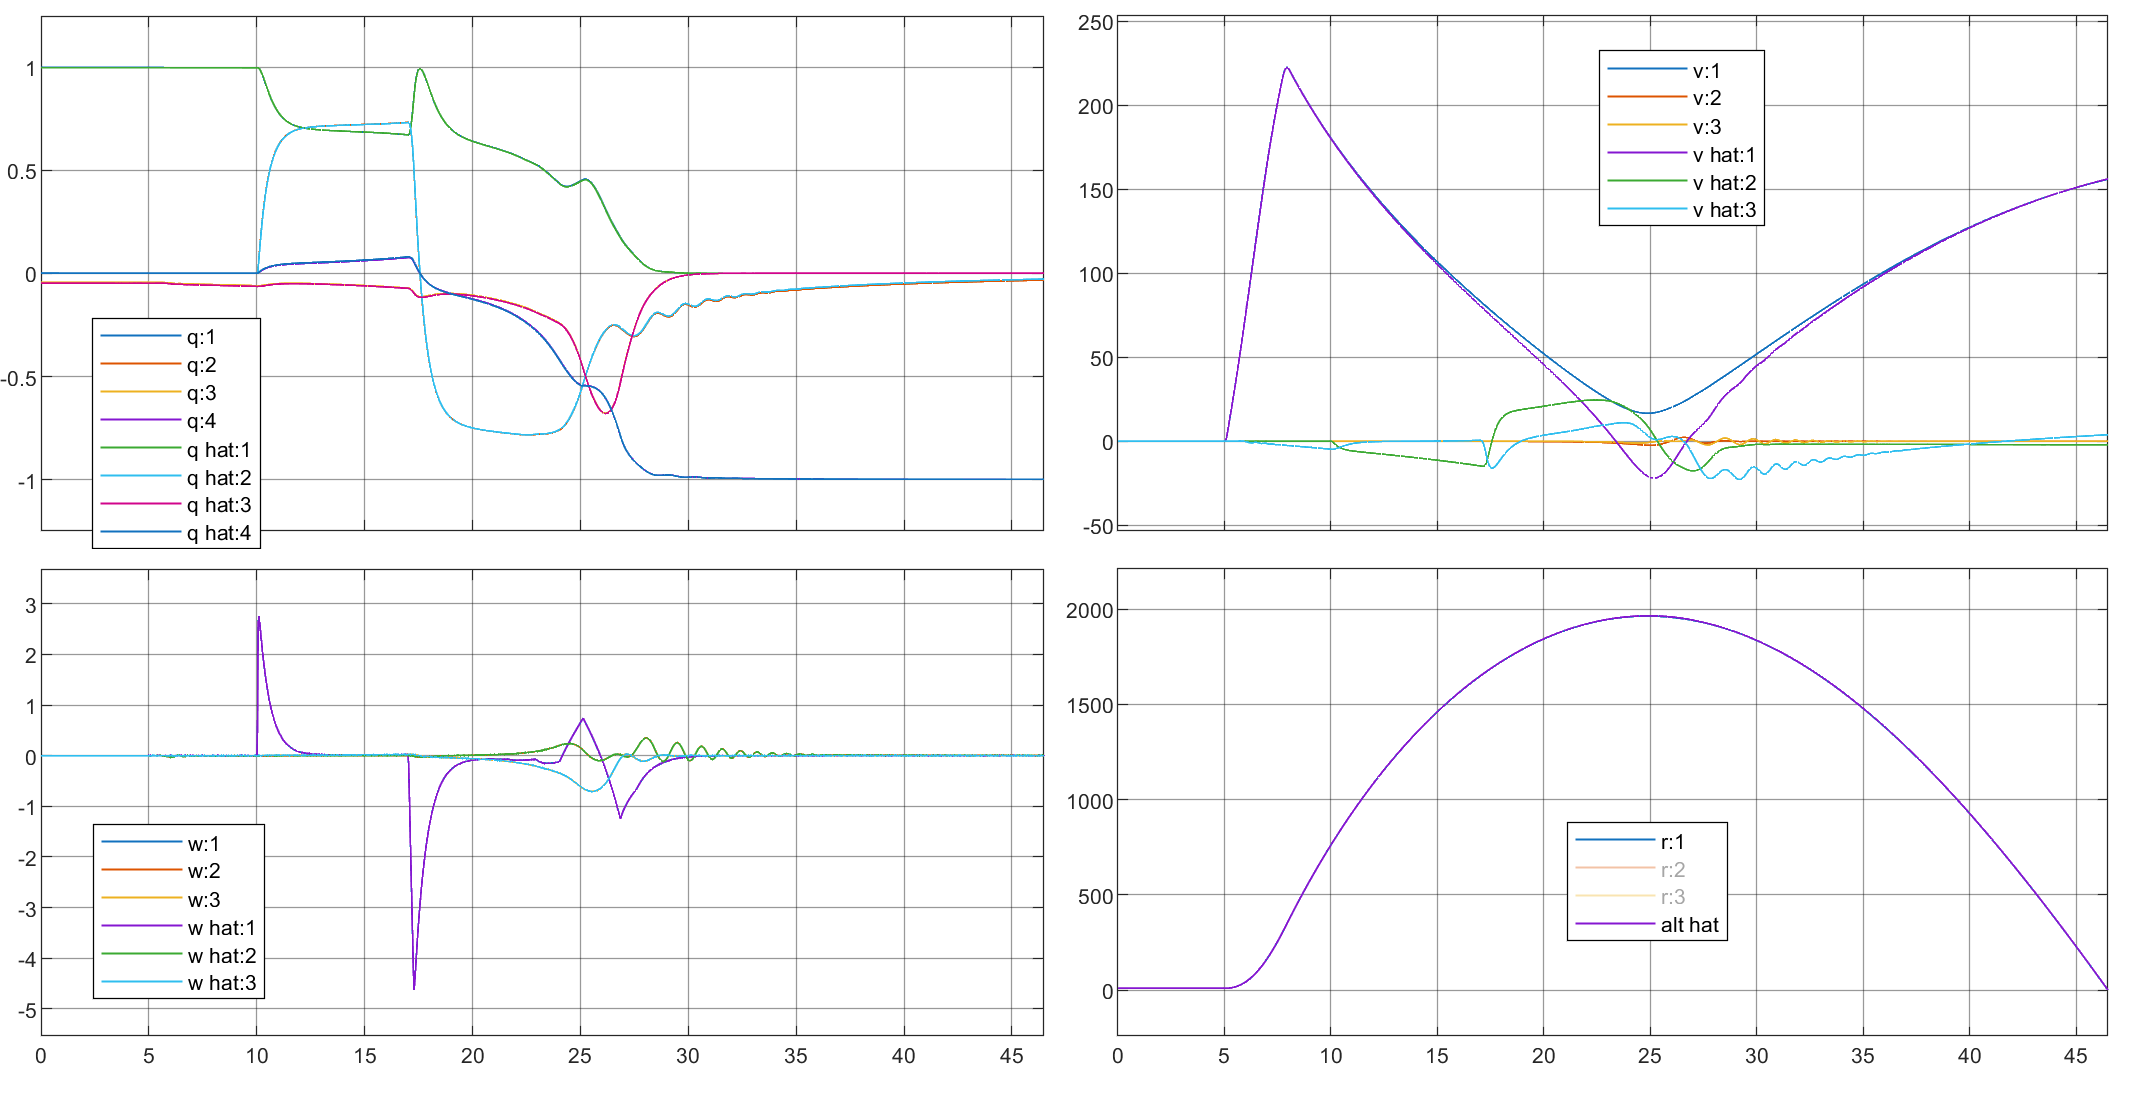
\includegraphics[width=\textwidth]{images-design/estimator-simulation.png}
    \caption[Closed-loop estimation responses]{Simulation responses of the closed-loop estimated states for the simulated testflight. Rocket is performing a step roll program at t=10s, t=17s, and t=24s. Outputs: Quaternion attitude $q, \, \hat q$ (Top Left),  Body rates $\omega, \, \hat \omega$ [rad/s] (Bottom Left), Body velocity $v, \, \hat v$ [m/s] (Top Right), Altitude $r_1, \, \hat {alt}$ [m] (Bottom Right).}
    \label{fig:estimator-response}
\end{figure}
Both the body rates and the altitude (bottom row) are estimated very well, which is due to the rate gyroscope measuring the state directly, and the barometer with an accurate atmosphere model having a direct coupling between measurement and state.
The attitude quaternion (top left) is also estimated quite well due to having both rate integrals and the magnetic field measurements. 
The gyroscope bias is determined on the launch pad (see Section \ref{sec:estimator-initialization}) which leads to low drift, and the magnetometer measurement further reduces perturbations from the true attitude.
The estimate is not perfect however, as can be seen in a slight deviation $q_2$ between 25s and 35s.\footnote{This .png makes it hard to see, the original plot has a higher resolution.}
The velocity estimate (top right) shows by far the largest deviation from the true values.
There is no measurement available for the velocity, so this estimate relies largely on accelerometer and gyroscope data.
While tuning, a strong coupling between velocity and attitude was noticed. 
As the rocket is essentially in free fall the entire flight, the accelerometer cannot measure the gravity vector, and any gravitational acceleration is modelled with the rocket attitude, see Equation \ref{eq:meas-veldot}.
Also, as the rocket is oriented vertical, the forward velocity is the change in altitude ($v_x \approx \dot {alt}$), so there is a strong coupling of forward velocity to the barometer data / its estimated altitude.
The velocity deviations become larger near apogee, where the rocket slows down and pitches over, before speeding up again.

\emph{Todo: insert responses of $\hat C_L$, $\hat \delta$}

\subsection{Implementation notes}
\label{sec:estimator-implementation}

\subsubsection{Computation frequency}
Computation time is an important factor in implementing the state estimation, as the discrete EKF process should be performed at $\omega_s \succapprox (20 \dots 30) \cdot \omega_c$ \cite{werner2021} to avoid the rocket crossover region, which is in frequencies around $ \omega_c \approx 5\mathrm{Hz}$.
The process frequency is chosen as $\omega_s = 200\mathrm{Hz}$ to leave some margin for error.

\subsubsection{Numerics}
The Jacobians $F$ and $H$ are computed numerically. 
Numerical methods for finite differentiation are shown in Section \ref{sec:numerical-jacobians}.

For the prediction step, numerical solvers are implemented to compute the solutions of the IVPs.
Here, \textit{explicit Euler} is used to compute a discrete state update.
%In this case these methods are \textit{Runge-Kutta(4)} for the state prediction and \textit{Heun's method} for the state covariance (see Section \ref{sec:numerical-integration}).
The methods are picked as a trade-off between accuracy and computational effort.

\subsubsection{Quaternions}
To ensure valid attitude quaternion operations, the norm of the quaternion has to be 1.
To ensure this unit norm, the quaternion is normalized after every operation changing its values, as $q = q/\mathrm{norm}(q)$ in the prediction model and after the correction step $\hat x_{k}^{+} = \hat x_{k}^{-} + K_{k} \left[ y_{k} - h(\hat x_{k}^{-}) \right]$, respectively.

\subsubsection{Projection}
As the controller expects not the full state $x$, but the roll state $x_R$ and the flight condition $x_{FC}$, some post-processing has to be performed.
This includes transforming the quaternion attitude to the roll angle, and computing the dynamic pressure from velocity and air data.

\subsection{Pad filter}
\label{sec:estimator-initialization}
This algorithm serves to compute accurate values for $\bar x_0$, and the sensor biases $b$.
While the rocket is stationary on the launch rail, the Pad filter runs in the Estimator loop instead of the EKF.
Shortly before liftoff, the Pad filter hands over the latest state estimate ($\bar x_0$) and the determined sensor biases to the EKF.
To get accurate values for the sensor biases, the Pad filter runs a lowpass filter with all the current sensor data $z_k$ and the already filtered data $s_k$ (start with $s_0 = \bm 0$)
\begin{align}
    s_{k+1} = \alpha z_k + (1-  \alpha) s_k
\end{align}
This should take place over a long time frame (longer than a minute) to attenuate any noise effects, or movement through plumbing or wind.
The gain $\alpha$ is chosen according to the allowable/expected time frame of initialization, a lower $\alpha$ results in a smoother, but slower converging signal ($\alpha$ is the time constant of this exponential discrete-time filter, the resulting shape is $e^{\alpha \, dt}$ with sampling time $dt$).

The IMUs should also be at a constant temperature, which shall\footnote{Or rather should, as this is not enforceable.} be the same as in flight (though some IMUs perform internal correction of the gyroscope temperature).
The biases and earth magnetic field are combined to the bias vector $b$.

As the filter runs while the rocket is stationary on the launch rail, several assumption can be made:
\begin{enumerate}
    \item The velocity of the rocket $v$ will be zero, and thus the altitude $l$ is constant.
    \item The acceleration of the rocket $\dot v$ will be zero.
    \item The body rates $\omega$ will be zero, and thus the attitude $q$ is constant.
\end{enumerate}
With the filtered data $s$, the state can be computed using the sensor models as follows:
\begin{enumerate}
    \item The accelerometer measurement will be the rotated gravity vector, so $S_A A = S^T g^G$. 
    No bias can be set for the individual axes, but the magnitude of the accelerometer measurement (part of $s_k$) should be $g$.
    
    \item The gyroscope bias $b_\Omega$ can be set to the filtered angular velocity (part of $s_k$) while the rocket is stationary.
    
    \item As the launch altitude is is known beforehand, any bias offset of the barometer $b_P$ can be corrected for with the atmosphere model. 
    
    \item The initial attitude will be close to, but not exactly upright.
    It is defined as yaw/pitch only, and thus can be computed uniquely from the accelerometer measurement.
    
    \item The magnetic field vector of the Earth $M_E^G$ can be computed from the filtered magnetic measurement $M$ (part of $s_k$) and by inverting the estimated initial attitude.
\end{enumerate}

\subsection{Hard calibration}
\label{sec:hard-calibration}
The orientation of all sensor frames ($S_\Omega, S_A, S_M$) to the rocket body must be determined \textit{well before} launch day.
Additionally, the position of the accelerometers $d_A$ to the dry center of gravity, and the the hard ($b_{HI}$) and soft ($B_{SI}$) iron biases for the magnetometer correction should be determined.

